\chapter{Results}
\label{cha:results}

%This chapter presents the results. Note that the results are presented
%factually, striving for objectivity as far as possible.  The results
%shall not be analyzed, discussed or evaluated.  This is left for the
%discussion chapter.

%In case the method chapter has been divided into subheadings such as
%pre-study, implementation and evaluation, the result chapter should
%have the same sub-headings. This gives a clear structure and makes the
%chapter easier to write.

%In case results are presented from a process (e.g. an implementation
%process), the main decisions made during the process must be clearly
%presented and justified. Normally, alternative attempts, etc, have
%already been described in the theory chapter, making it possible to
%refer to it as part of the justification.

In this chapter the results are described.
First, the outcome from the exploratory study is presented, followed by the different experiments.
The first experiment, filtering out invalid reports, presents the evaluation of the topic model and k-means model used to filter out the reports, as well as the specific topics and clusters used in the process.
In the second one, the methods considered and the decisions behind which ones that were appropriate are presented.
Finally, the last section goes through the result of evaluating the different active learning techniques.

\section{Exploratory Study}

The goal with the exploratory study was to acquire a better understanding of the data, how it was structured and what kind of information might be extracted from it.
[FIGURE FROM METHOD] displayed popular terms from a subset of the topics obtained from the topic model.
Certain fields such as the cancelled field did not seem to be very reliable. 
Reports that clearly explained a situation where the patient had been transferred to another hospital, or for another reason not having performed an examination, still described a situation where the cancelled field was set to ``false''.
After further manual analysis it was clear that the vast amount of invalid reports were contained within a few topics, something that is used in the first research question.
The evaluation of more concrete relationships were done within the context of that experiment, and is presented in Section~\ref{sec:exp1-result}.

The word2vec model produced results that allowed for synonyms to be detected.
By doing this, 420 pairs were detected.
The vast majority of these were names, medical terms that (some of which the author was unable to evaluate, and therefore excluded) as well as words that are used in similar contexts, which includes opposites like ``left'' and ``right''.
Disregarding these, the synonyms and misspellings that were decided for use in the final system can be seen in Table~\ref{tab:synonyms}.
The original value was replaced with the new one in the final system.

\begin{table}
    \centering
    \begin{tabular}{|ccc|}
        \hline
        \textbf{Original} & \textbf{Replacement} & \textbf{Type} \\
        \hline
        ordinärt & normalt & synonyms \\
        ej & inte & synonyms \\
        avbeställd & avbokad & synonyms \\
        avebställd & avbokad & misspelling + synonym \\
        belsutat & beslutat & misspelling \\
        måttliga & lätta & synonyms \\
        pat & patient & short \\
        pt & patient & short \\
        pateint & patient & misspelling \\
        akuten & akutmottagningen & misspelling \\
        us & undersökning & short \\
        \hline
    \end{tabular}
    \caption{The synonyms, misspellings and shorts found in the data that the author could with assert with confidence.}
    \label{tab:synonyms}
\end{table}

In order to identify names from this word2vec model, it was plotted using the an interactive plot that allowed for exploring the data.
Since names are commonly used in similar contexts, they would have similar attributes in the word embedding model.
Figure~\ref{fig:word2vec-overview} and Figure~\ref{fig:word2vec-names} show how this was done.
Given that the names got similar coordinates in the plot, identifying the section with names allowed for identification of a lot of the names used in the reports.

\begin{figure}
    \centering
    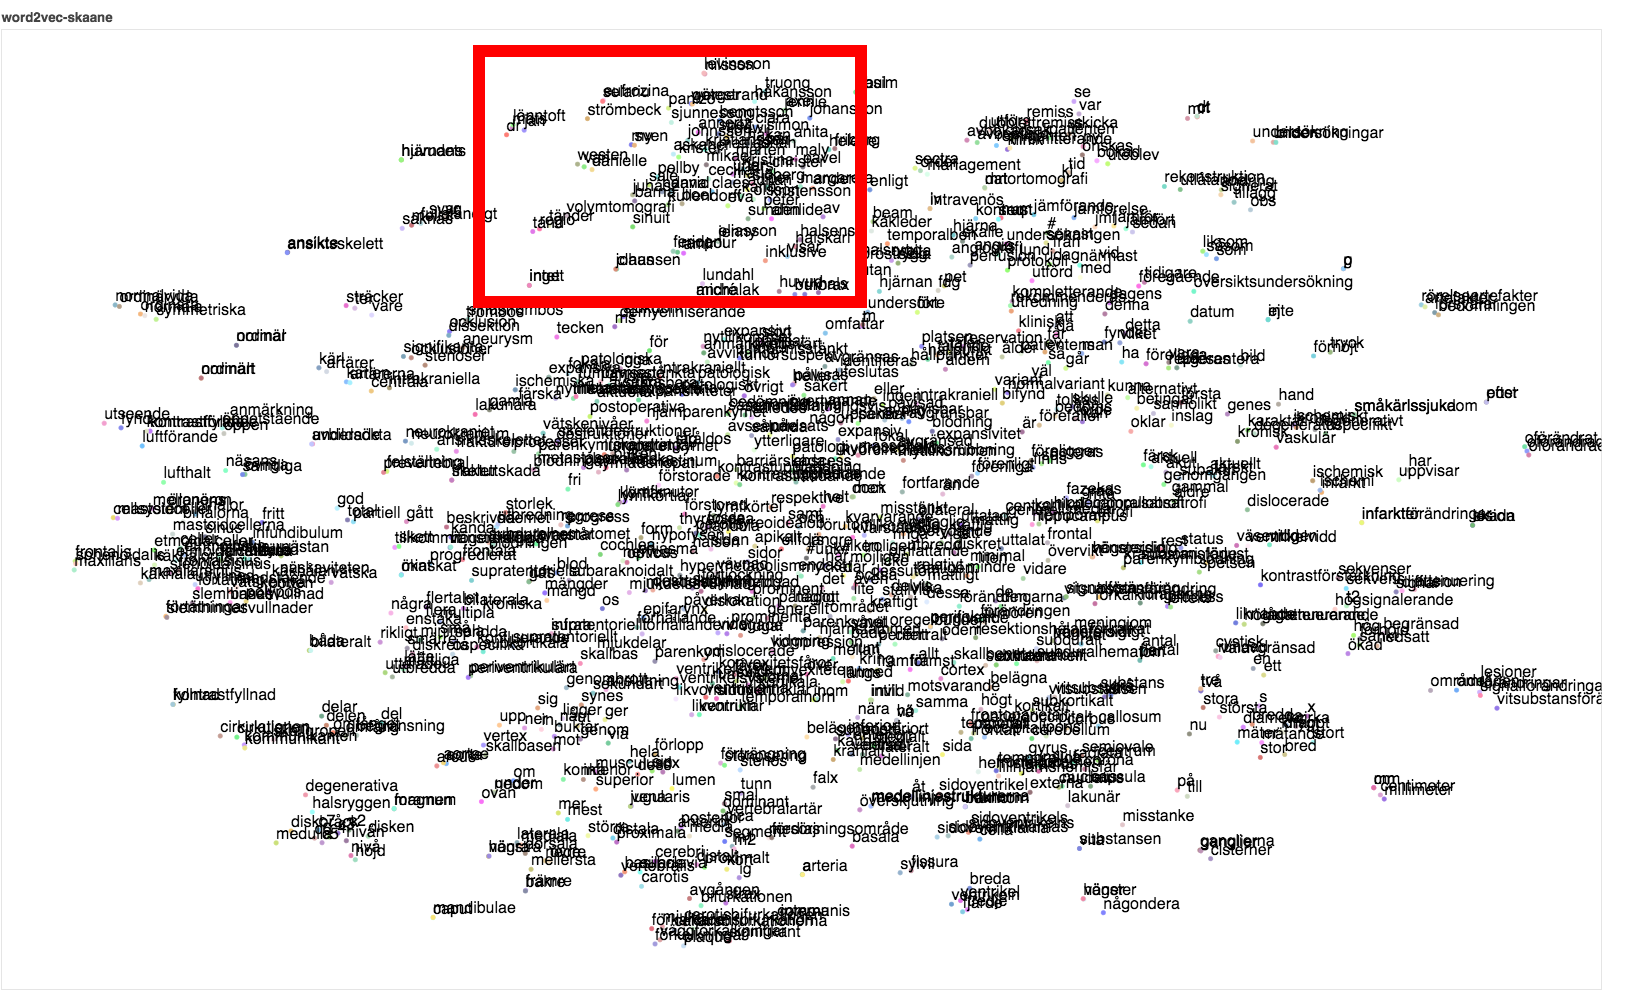
\includegraphics[scale=0.25]{figures/word2vec-overview.png}
    \caption{A 2D plot of the full word2vec plot. Given the amount of terms used there is a lot to analyze.}
    \label{fig:word2vec-overview}
\end{figure}

\begin{figure}
    \centering
    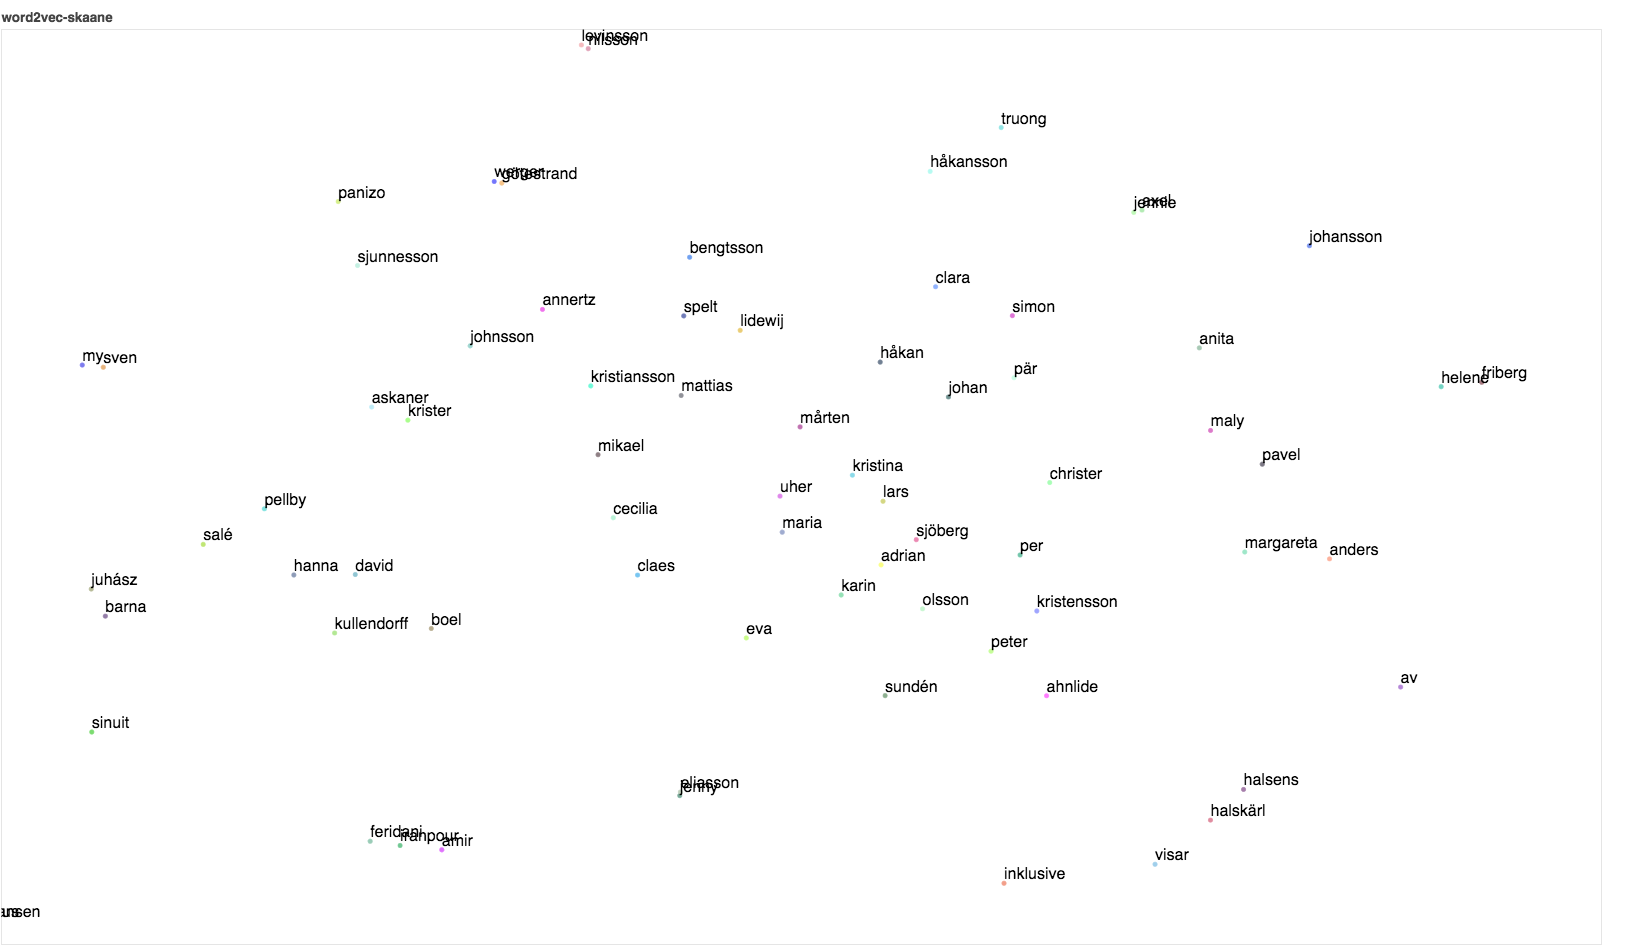
\includegraphics[scale=0.25]{figures/word2vec-names.png}
    \caption{A 2D plot of the zoomed in word2vec plot. Most of the values here are names. This represents the red box zoomed in from Figure~\ref{fig:word2vec-overview}}.
    \label{fig:word2vec-names}
\end{figure}

\section{EXPERIMENT 1}\label{sec:exp1-result}

The distribution of the most likely topics for the invalid reports can be seen in [FIGURE].
As can be seen, topic 17 and topic 34 were the most likely.
They were combined by ..... (SPECIFICS FOR THE CHOSEN MODEL).

The distribution over the invalid reports by cluster can be seen in [FIGURE].
The selected cluster was 25 based on the overwhelming majority.

\section{EXPERIMIENT 2}

WIRTE THIS
However, the relationship is not clear enough so that a cluster or topic could simply be mapped to a certain label.
The resulting plot can be seen in Figure~\ref{fig:categories-lda-50}.

\begin{figure}
    \centering
    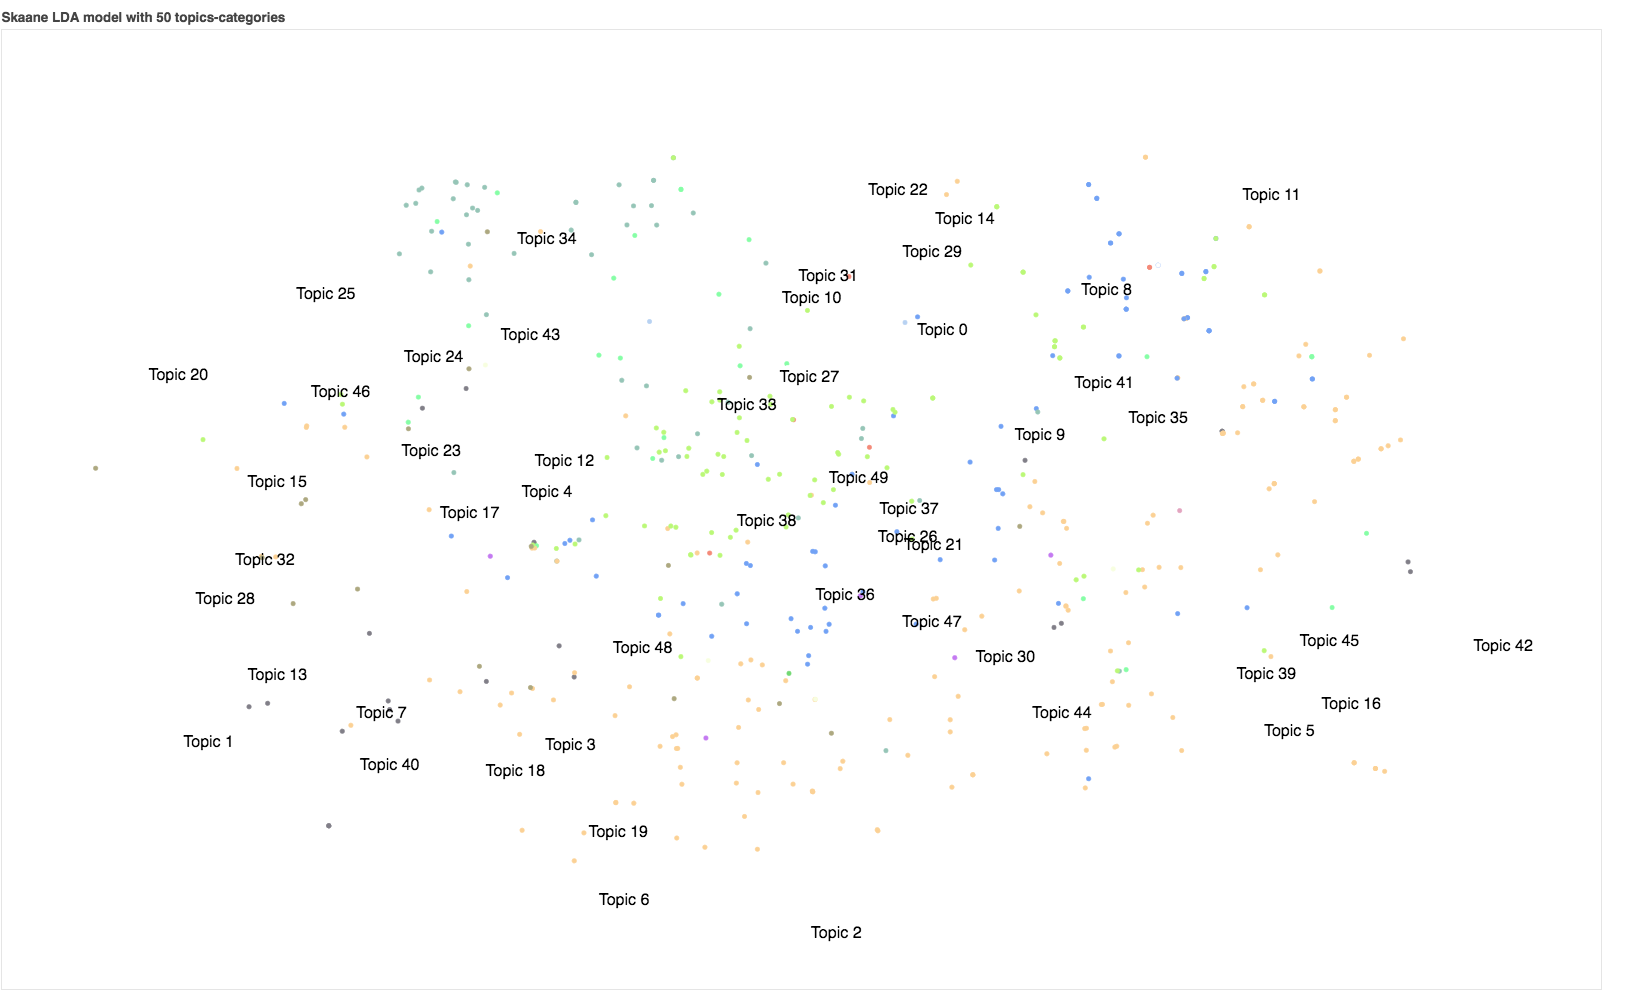
\includegraphics[scale=0.35, angle=270]{figures/categories-lda-50.png}
    \caption{The labeled data points plotted in 2D, and colored based on the first label in alphabetical order.}
    \label{fig:categories-lda-50}
\end{figure}

Since there was a pattern some active learning approaches using different forms of clustering, such as Dasgupta et al\@'s approach using hierarchical clustering~\cite{dasgupta2008hierarchical}.
However, it is made for the single-label case with no obvious way of extending the technique into multi-label.
The same applies to the density based technique suggested by Attenberg et al\@.~\cite{attenberg2013class}.